%%%%%%%%%%%%%%%%%%%%%%%%%%%%%%%%%%%%%%%%%%%%%%%%%%%%%%%%%%%%%%%%%%
%%        mmm  mmmmmm mm   m        m    m mmmmmm m             %%
%%      m"   " #      #"m  #        #    # #      #  #          %%
%%      #   mm #mmmmm # #m #        #    # #mmmmm "mm#mm        %%
%%      #    # #      #  # #  """   #    # #         #          %%
%%       "mmm" #mmmmm #   ##        "mmmm" #mmmmm    #          %%
%%                                                              %%
%%                                                              %%
%%                                                              %%
%%      Grundlagen der Elektrischen Netzwerke, UE               %%
%%      Gruppe 5, Team F                                        %%
%%      Authors: Severin Wolf, Maximilian Seidler.              %%
%%%%%%%%%%%%%%%%%%%%%%%%%%%%%%%%%%%%%%%%%%%%%%%%%%%%%%%%%%%%%%%%%%
\documentclass[a4paper]{article}
\usepackage{amsmath}
\usepackage[utf8]{inputenc}
\usepackage[T1]{fontenc}
\usepackage[english]{babel}
\usepackage{geometry}
\usepackage{graphicx}
\usepackage{tikz}
\usepackage{listings}
\geometry{a4paper,left=3cm,right=2cm, top=2cm, bottom=2cm} 
\usepackage[EFvoltages, european, straightvoltages]{circuitikz}

%tikz
\ctikzset{resistor = european}
\usetikzlibrary{decorations.pathreplacing}

%no paragraph indent
\setlength{\parindent}{0pt}

%for math, that does not fit
\renewcommand*{\arraystretch}{1.3}
\newcommand\scalemath[2]{\scalebox{#1}{\mbox{\ensuremath{\displaystyle #2}}}}

\newcommand\blfootnote[1]{%
	\begingroup
	\renewcommand\thefootnote{}\footnote{#1}%
	\addtocounter{footnote}{-1}%
	\endgroup
}

% upright differenzial symbol with good spacing included!!!
\makeatletter
\providecommand*{\diff}%
	{\@ifnextchar^{\DIfF}{\DIfF^{}}}
\def\DIfF^#1{%
	\mathop{\mathrm{\mathstrut d}}%
		\nolimits^{#1}\gobblespace
}
\def\gobblespace{%
	\futurelet\diffarg\opspace}
\def\opspace{%
	\let\DiffSpace\!%
	\ifx\diffarg(%
		\let\DiffSpace\relax
	\else
		\ifx\diffarg\{%
			\let\DiffSpace\relax
		\else
			\ifx\diffarg\{%
				\let\DiffSpace\relax
			\fi\fi\fi\DiffSpace}

\begin{document}
\pagestyle{empty} \enlargethispage*{25cm}\samepage{
\vspace*{-3cm}
\begin{center}
\begin{minipage}[!h]{16cm}
\hspace*{0.2cm}

\includegraphics[width=3.3cm]{./Figures/igte_logo}
\begin{tabular}{p{8cm}}
\vspace{0.2cm}
\centering{
\Large Institute of Fundamentals and Theory in
 Electrical Engineering\\
Graz University of Technology\\
~\\}
\end{tabular}

\includegraphics[width=3.3cm]{./Figures/TUG_logo}
\end{minipage}
		\Large
		\textbf{Fundamentals of Electrical Circuits} \vspace*{0.5cm}\\
		\textbf{4. Homework}\\Transient response
		\vspace*{0.5cm}
		
		\large
		15 April 2021
	\end{center}}
	
	%%%%%%%%%%%%%%%%%%%%%%%%%%%%%%%%%%%%%%%%%%%%%%%%%%%%%%%%%%%%%%%%%%%%
	%%%%%%%%%%%%%%%%%%%%%%%%%%%%%%%%%%%%%%%%%%%%%%%%%%%%%%%%%%%%%%%%%%%%
	\section*{Assignment 1}
	\begin{enumerate}
		\item The  expression for the current $i_L(t)$ for $t\geq0$ should be found:
		\begin{itemize}
			\item Apply the general solution for transient response $\mathbf{x(t) = x_f + [x_0 - x_f ] \cdot e^{-\frac{t-t_0}{\tau}}}$ in order to calculate the expression for $i_L(t)$ for $0 \leq t \leq 2 \tau_1$. The value of $i_L(2 \tau_1)$ should be used as initial condition for the coil for $t \geq 2 \tau_1$. (0.5P)
						
			\item At $t = 2 \tau_1$ both switches $S_1$ and $S_2$ close instantaneously. Apply KCL and KVL for the remaining circuit to derive the necessary mesh and node equations. Use the $\textbf{\textit{i}}-\textbf{\textit{u}}$ relationships at the resistors, the capacitor and the coil in order to derive the homogeneous second order differential equation describing the current $i_L(t)$. \\\textbf{Hint:} $i_L'' + 2 \delta i_L' + \omega_0^2 i_L = 0$ (1P)
	
			\item Calculate the value of the parameters $\delta,\omega_0$ and $\Omega_d$. Is this specific circuit overdamped, underdamped or critically damped? (0.5P)
			
			\item  Solve the second order differential equation describing $i_L(t)$ by using the correct \textit{Ansatz} for this case. (1P)
			\begin{itemize}
				\item Use the appropriate \textit{Ansatz} depending on the case
				\item Solve the initial value problem for the corresponding initial conditions. Explain your thoughts.
			\end{itemize}				
		\end{itemize}
	
		\item Plot the current through the inductor in Matlab for $0s\leq t<10ms$. (1P)
		
		\item Do a simulation of the circuit in LTspice and compare the results. Plot the current $i_L(t)$ and the voltage $u_L(t)$ at the coil between $0s\leq t<10ms$. (1P)
		\\\textbf{Hint:} To set the initial conditions in LTspice use the spice-directive \textbf{.ic} for example \textbf{.ic I(L1)=50m} \\
		for voltages at capacitors it works best to define the initial voltages of the specific nodes around the capacitor \textbf{.ic V(n003)=-5} therefor you have to calculate the voltages at this nodes at the beginning first.(a little bit annoying in LTspice)
		
		
	\end{enumerate}
	
	\vspace*{8cm}
	
\blfootnote{Deadline: 22 April 2021; \qquad presentation: Group 4}

\newpage	
\vspace*{4cm}
\begin{figure}[h!]
		\centering
			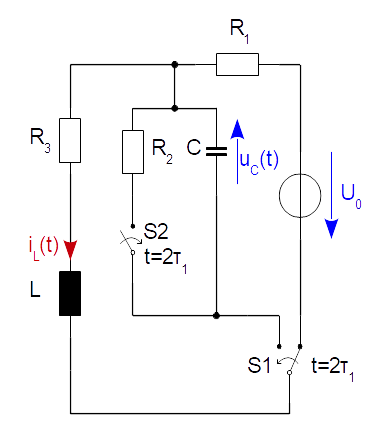
\includegraphics[width = 350pt]{./Figures/homework04_circuit.png}
			\caption{Given circuit}
			\label{fig:circuit_hw04}
\end{figure}

\vspace*{2cm} \subsection*{Values:}
$R_1 = 50\Omega$ \qquad $R_2 = 200\Omega$ \qquad $R_3 = 50\Omega$ \qquad $C = 10\mu F$ \qquad $L = 100mH$ \qquad $U_0 = 10V$ \newline 
$i_L(t=0ms)=I_{L,0}=50mA$ \qquad $u_C(t=0ms) = U_{C,0} = 15V$

\newpage
\section{Solution}
\subsection{Analytical calculations}
Circuit for $0 \leq t \leq 2\tau_1$:

\begin{figure}[h!]\centering
	\begin{circuitikz}[scale=0.75, transform shape]
		\draw(0,0)
		to[short](0,1)
		to[L, l=$L$, v<=$U_{L}$](0,4)
		to[short, i<=$i_L(t)$, color=red](0,5)
		to[short](1,5)
		to[R, l=$R_{13}$, v<=$U_{R_{13}}$](4,5)
		to[short](5,5)
		to[short](5,4)
		to[V, v=$U_0$, color=blue](5,1)
		to[short](5,0)
		to[short](0,0);
	\end{circuitikz}
\end{figure}
$R_{13} = R_1 + R_3$
\begin{align*}
	i_L(t) =& x_f + [x_0 - x_f ] \cdot e^{-\frac{t-t_0}{\tau}}\\
	i_L(t) =& \mathrm{final \; currenrt + [initial \; currenrt - final \; current] \cdot e^{-\frac{t-starttime}{\tau}}}\\
	x_0 =& i_{L_0} = 50mA\\
	x_f =& i_{L_f} = \frac{U_0}{R_{13}}, \;\;\;\; \text{L becomes a short after a very long time} (>5\tau)\\
	t_0 =& 0\\
	\tau =& \frac{L}{R_{13}}\\
	i_L(t) =& \frac{U_0}{R_{13}} + \left[50mA - \frac{U_0}{R_{13}} \right] \cdot e^{-\frac{t}{\frac{L}{R_{13}}}}\\
\end{align*}

Circuit for $t \geq 2\tau_1$:
\begin{figure}[h!]\centering
	\begin{circuitikz}[scale=0.75, transform shape]
		\draw(0,0)
		to[short, *-](0,1)
		to[L, l=$L$, v<=$u_{L}(t)$](0,4)
		to[short, i<=$i_L(t)$, color=red](0,5)
		to[short](0,6)
		to[R, l=$R_{3}$, v<=$u_{R_{3}}(t)$](0,9)
		to[short, -*](0,10);
		\draw(5,0)
		to[short, i<=$i_{R_2}(t)$, color=red](5,2)
		to[R, l=$R_{2}$, v<=$u_{R_{2}}(t)$](5,8)
		to[short, -*](5,10);
		\draw(10,0)
		to[short, i<=$i_{C}(t)$, color=red](10,2)
		to[C, l=$C$, v<=$u_{C}(t)$](10,8)
		to[short, -*](10,10);
		\draw(0,10) to[short](10,10);
		\draw(0,0) to[short, -*](5,0) to[short, -*](10,0);
	\end{circuitikz}
\end{figure}

$t^{~} = t - 2\tau_1$

\begin{align*}
	m_1&: u_C(t) = u_{R_2}(t)\\
	m_2&: u_{R_3}(t) + u_L(t) = u_{R_2}(t)\\
	n&: i_L(t) + i_{R_2}(t) + i_C(t) = 0\\
\end{align*}
\begin{align*}
	i_L + i_{R_2} + i_C(t) = 0\\
	i_L + \frac{u_{R_2}}{R_2} + Cu_C' = 0\\
	i_L + \frac{u_{R_3} + u_L}{R_2} + C(u_{R_3} + u_L)' = 0\\
	i_L + \frac{u_{R_3}}{R_2} + \frac{Li_L'}{R_2} + C(u_{R_3} + Li_L')' = 0\\
	i_L + \frac{i_LR_3}{R_2} + \frac{Li_L'}{R_2} + C(i_LR_3 + Li_L')' = 0\\
	i_L \left(1 + \frac{R_3}{R_2} \right) + \frac{Li_L'}{R_2} + CR_3i_L' + CLi_L'' = 0\\
	CLi_L'' + i_L'\left( \frac{L}{R_2} + CR_3 \right) + i_L \left(1 + \frac{R_3}{R_2} \right) = 0\\
	i_L'' + i_L'\left( \frac{1}{R_2C} + \frac{R_3}{L} \right) + i_L \left(\frac{1}{CL} + \frac{R_3}{R_2CL} \right) = 0\\
\end{align*}
\begin{align*}
	2\delta = \left( \frac{1}{R_2C} + \frac{R_3}{L} \right)\\
	\omega_0^2 = \left(\frac{1}{CL} + \frac{R_3}{R_2CL} \right)\\
\end{align*}
educated guess:
\begin{align*}
	i_L &= e^{\lambda t},&
	i_L' &= \lambda e^{\lambda t},&
	i_L'' &= \lambda^2 e^{\lambda t}\\
\end{align*}
\begin{align*}
	\lambda^2 e^{\lambda t} + 2\delta\lambda e^{\lambda t} + \omega_0^2 e^{\lambda t} 
	= e^{\lambda t}(\lambda^2 + 2\delta\lambda + \omega_0^2) = 0\\
\end{align*}
characteristic equation:
\begin{align*}
	\lambda^2 + 2\delta\lambda + \omega_0^2 = 0\\
	\lambda_{1,2} = -\delta \pm \sqrt{\delta^2 - \omega_0^2}
\end{align*}


\end{document}
